\documentclass[10pt,a4paper]{article}
\usepackage[utf8]{inputenc}
\usepackage[T1]{fontenc}
\usepackage{lmodern}
\usepackage[margin=1.5cm, top=1.4cm, bottom=1.4cm]{geometry}
\usepackage{hyperref}
\usepackage{enumitem}
\usepackage{titlesec}
\usepackage{xcolor}
\usepackage{graphicx}

\definecolor{accent}{HTML}{00686E}
\hypersetup{colorlinks=true, urlcolor=accent, linkcolor=accent}
\pagenumbering{arabic}
\setlength{\parindent}{0pt}

\titleformat{\section}{\large\bfseries\color{accent}}{}{0em}{}[\vspace{-0.6em}\rule{\textwidth}{0.8pt}]
\titlespacing{\section}{0pt}{7pt}{4pt}

\newcommand{\role}[4]{%
  \textbf{#1} \hfill \textbf{#2}\\[1pt]%
  \textit{#3} \hfill \textit{#4}\\[2pt]%
}
\setlist[itemize]{leftmargin=1.2em, itemsep=1.5pt, topsep=2pt, parsep=0pt}

\begin{document}

% ================= HEADER =================
\begin{minipage}[c]{0.80\textwidth}
  {\Huge\bfseries Prabhavit Gupta}\\[3pt]
  {\color{accent}\large AI Engineer: Generative AI, RAG Architectures \& Production LLM Systems}\\[6pt]
  {\footnotesize +39 351 610 7807 ~$\vert$~
  \href{mailto:prabhavitg@gmail.com}{prabhavitg@gmail.com} ~$\vert$~
  \href{https://www.linkedin.com/in/prabhavit/}{linkedin.com/in/prabhavit} ~$\vert$~
  \href{https://github.com/prab-gupta}{github.com/prab-gupta} ~$\vert$~
  Venice, Italy (EU Permanent / Remote Freelance Ready)}
\end{minipage}\hfill
\begin{minipage}[c]{0.18\textwidth}
  \raggedleft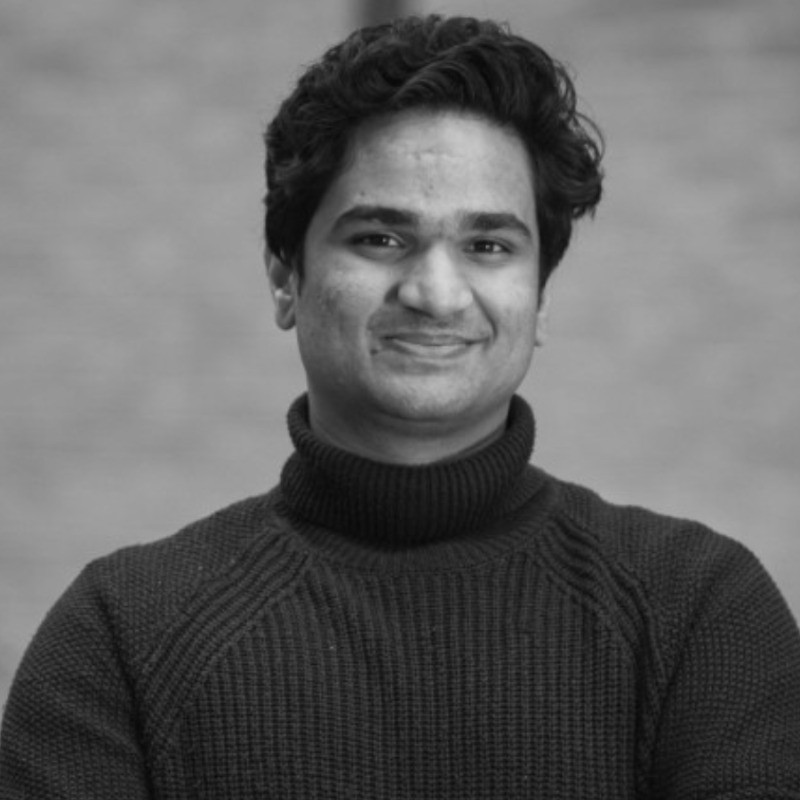
\includegraphics[width=2.0cm]{photo.jpg}
\end{minipage}
\vspace{-2pt}

% ================= SUMMARY =================
\section{Summary}
AI Solutions \& Automation Engineer with 3 years of hands-on production experience architecting, deploying, and maintaining production-ready Generative AI systems, RAG pipelines, and enterprise automation workflows. Proven track record turning complex enterprise requirements into scalable LLM applications, integrating multi-modal APIs, vector search datastores, and cloud infrastructure across European client environments. Deep practical experience implementing evaluation harnesses, managing token optimization, and establishing CI/CD and MLOps deployment standards. Holder of an EU Long-Term Residence Permit (permanent unrestricted EU work authorization across all EU member states, no sponsorship required); based in Venice, Italy and available immediately for remote freelance contracts and European on-site travel.

% ================= TECHNICAL EXPERTISE =================
\section{Technical Expertise}
\begin{itemize}
  \item \textbf{Generative AI \& LLM Applications:} LLM APIs (OpenAI, Anthropic), RAG architectures, semantic retrieval, embeddings, vector indexing, prompt engineering, context management, structured JSON outputs, transcript evaluation harnesses.
  \item \textbf{Software Development \& Integration:} Python, TypeScript, Node.js, RESTful APIs, webhook consumers, data ingestion and transformation pipelines, PostgreSQL schema modeling, Redis asynchronous queues.
  \item \textbf{Cloud \& MLOps Practices:} Cloud environments (Azure, AWS), Docker containerization, CI/CD pipelines, Git version control, observability and trace monitoring, automated regression testing with Playwright.
  \item \textbf{Workflow Automation \& Enterprise Delivery:} n8n orchestration, third-party system synchronization, SLA compliance, technical documentation, cross-functional stakeholder collaboration.
  \item \textbf{Languages \& Work Authorization:} English (C1 Professional, fluent), Hindi (Native), Italian (Beginner). EU Long-Term Residence Permit (unrestricted EU work authorization across all EU member states, no sponsorship required).
\end{itemize}

% ================= EXPERIENCE =================
\section{Experience}

\role{\href{https://flowspace.co}{FlowSpace.co}}{Mar 2024 - Aug 2026}{Lead Developer \& AI Systems Architect}{London, UK (remote)}
\begin{itemize}
  \item Designed and operated production customer-facing AI agents for a marketplace platform serving 4,500+ active enterprise users, handling complex inquiries against live platform data and APIs.
  \item Implemented automated document and data parsing pipelines with LLM extraction, converting unstructured partner data into validated JSON schemas and expanding live platform inventory.
  \item Built human-in-the-loop escalation workflows and multi-step reasoning chains with strict tool constraints, ensuring zero ungrounded responses in customer-facing flows.
  \item Evaluated system prompts and tool schemas against real production transcripts, systematically lowering edge-case error rates and measuring response quality against ground-truth validation datasets.
  \item Maintained resilient backend integrations with TypeScript/Node.js and PostgreSQL, implementing asynchronous queues and automated retries for high-throughput reliability.
  \item Built automated end-to-end integration and regression test suites with Playwright, ensuring API contract validity and zero regressions across continuous release cycles.
\end{itemize}

\role{Urlink}{Apr 2025 - Jul 2025}{Project Manager \& Solutions Developer (Freelance)}{Barcelona, Spain (remote)}
\begin{itemize}
  \item Led technical discovery and implementation of customized web solutions and automated data processing pipelines for client platforms.
  \item Built automated data ingestion and transformation services connecting third-party APIs to PostgreSQL datastores, maintaining high data freshness and integrity.
  \item Delivered interactive functional prototypes to validate user flows and technical requirements prior to sprint execution, accelerating cycle times.
\end{itemize}

\role{Independent Technical Consultant}{Aug 2023 - Feb 2024}{AI Automation \& Integration Developer}{Venice, Italy}
\begin{itemize}
  \item Designed, deployed, and supported tailored LLM integrations, document-parsing pipelines, and webhook orchestration workflows for European clients using Python, TypeScript, and n8n.
  \item Replaced fragile manual data entry workflows with automated sync pipelines featuring structured error handling, retry policies, and alerting.
  \item Documented system architectures and delivered technical walkthroughs, ensuring smooth client adoption and high operational reliability.
\end{itemize}

% ================= EDUCATION =================
\section{Education}
\role{Ca' Foscari University of Venice}{2020 - 2024}{BA in Philosophy, International Studies and Economics}{Venice, Italy}
\begin{itemize}
  \item Rigorous training in formal logic, analytical problem solving, systems analysis, and macroeconomic decision models.
\end{itemize}

\end{document}
